\documentclass[10pt,letterpaper]{article}
\usepackage[margin=1in]{geometry}
\usepackage[T1]{fontenc}
\usepackage{lmodern,microtype}
\usepackage{amsmath,amssymb,booktabs,longtable,array}
\usepackage{xcolor,listings}
\usepackage{tikz}
\usetikzlibrary{arrows.meta,positioning}
\usepackage[colorlinks=true,linkcolor=blue!50!black,urlcolor=blue!50!black,citecolor=blue!50!black]{hyperref}
\hypersetup{pdftitle={Adapting Volta to AMD GPUs},pdfauthor={GPU Kernel Verifier contributors}}
\newcommand{\code}[1]{\texttt{\detokenize{#1}}}
\newcommand{\repo}[2]{\href{https://github.com/harsh-nod/ptx_verifier/blob/main/#1}{#2}}
\newcommand{\accept}{\textsc{Accept}}
\newcommand{\reject}{\textsc{Reject}}
\newcommand{\unknown}{\textsc{Unknown}}
\lstset{basicstyle=\small\ttfamily,breaklines=true,columns=fullflexible,
  keepspaces=true,frame=single,rulecolor=\color{black!20},showstringspaces=false}
\setlength{\emergencystretch}{2em}

\title{Adapting Volta to AMD GPUs:\\Native Execution Semantics and Target-Specific Safety Checking}
\author{GPU Kernel Verifier contributors}
\date{Technical report \textemdash{} October 2026}

\begin{document}
\maketitle
\begin{abstract}
Volta combines symbolic execution of GPU kernels with mathematical output
equivalence. Extending that approach from NVIDIA PTX to native AMD assembly
requires a new execution model and new safety obligations. This report describes
the implementation in GPU Kernel Verifier for selected gfx942, gfx950 and gfx1250
instruction profiles. The main changes are an AMDHSA-aware frontend and typed
lowering path; wave-level execution with explicit register, byte and ABI
definedness; target-specific event records for asynchronous memory, matrix
operations and synchronization; independent graph checks; and shared output and
result contracts across the CLI and Python interfaces. The expression and
equivalence layers remain largely reusable. Compiler fixtures, exact output
projections and harmful mutations provide implementation evidence, while
independent numerical drivers address a different question from symbolic
equivalence. The implementation is an experimental bug-finding tool. This report
does not extend Volta's formal results to AMD hardware or establish complete ISA,
floating-point or whole-grid verification.
\end{abstract}

\section{Problem and scope}
\label{sec:scope}

Volta's original setting is equivalence checking for structured GPU kernels:
thread geometry, pointer targets and branch decisions are statically resolvable,
while arithmetic data can remain symbolic. The original work presents formal
results for its specified language and arithmetic fragment~\cite{volta}. Those
results are background for this implementation, rather than a proof of the
native AMD extension described here.

The practical goal is to analyze the assembly that an AMD compiler actually
emits, detect synchronization and storage hazards in its supported execution
profile, and compare its complete mathematical outputs with a specification or
another kernel. Running the analyzer on checked-in assembly requires a CPU;
ROCm and a device are needed for fixture regeneration and independent device
experiments, respectively.

The implementation uses three target profiles. gfx942 and gfx950 use wave64
execution with selected CDNA3/CDNA4 MFMA forms. gfx1250 uses wave32 execution,
selected WMMA forms and separate completion and barrier protocols. These names
identify implemented subsets. They do not imply support for every instruction,
target alias, operand tuple or execution mode. Public ISA and compiler sources
provide the semantic references~\cite{cdna3,cdna4,llvmabi,llvmhazard,llvmsync,llvmdma}.

The analyzed launch selects workgroup $(0,0,0)$. Its configured grid remains an
input because kernels can derive dimensions from it. Addresses and control
decisions must become concrete. Floating arithmetic uses a mathematical-real
abstraction; encoded storage and selected concrete integer operations have
separate rules. The resulting claims concern that configured execution and its
reported assumptions, rather than arbitrary launches or physical rounding.

\paragraph{Implementation reference.}
The accompanying source tree is the executable specification for this report.
The PTX-only comparison baseline is repository commit \code{e8f8199}; the
\repo{docs/architecture.md}{architecture guide} describes current module
boundaries. The experimental \code{volta_amd_analysis} scaffold is distinct from
the \code{volta_amdgpu_analysis} backend used by the CLI and Python. External
semantic and compiler revisions are pinned separately in
\repo{tests/gfx1250/fixtures/semantic-references.json}{the semantic reference manifest}.
No private architectural material or machine-specific observations are needed
to understand the model in this report.

\section{What had to change}
\label{sec:changes}

An instruction-name translation is insufficient. The same arithmetic operation
can have different physical participants, register storage, completion rules and
synchronization obligations. Table~\ref{tab:changes} distinguishes the reusable
components from the AMD-specific work.

\begin{table}[ht]
\centering\small
\begin{tabular}{p{0.19\linewidth}p{0.34\linewidth}p{0.36\linewidth}}
\toprule
Layer & Reused contract & AMD extension \\
\midrule
Frontend & Source locations, launch inputs and diagnostics & Native assembly grammar,
kernel descriptors, AMDHSA metadata, globals and exact target validation \\
Execution & Symbolic expressions and output extraction & Wave PC, SGPR/VGPR state,
EXEC/VCC/SCC, byte-defined memory and native matrix layouts \\
Event graph & Typed events, footprints, terminal states and provenance & Wave operands,
memory issues, counter charges, register leases, matrix delays and barrier state \\
Safety & Independent pass/fail/unknown reports & Target-selected completeness,
readiness, barrier and memory-conflict checks \\
Equivalence & Specification language, expression DAG and algebraic comparison & Exact
native output projections, encoded-data boundaries and scalable DAG handling \\
Interfaces & CLI, Python and event viewer & Backend/target routing, native launch
premises, typed failures and wave-aware display \\
Validation & Positive and negative tests & Genuine compiler output, native mutations,
source pins, independent layout and device oracles \\
\bottomrule
\end{tabular}
\caption{Responsibilities retained and added by the AMD extension. A shared data
structure does not imply a shared target safety rule.}
\label{tab:changes}
\end{table}

\subsection{A boundary between execution and checking}

The native analyzer constructs artifacts rather than issuing a verification
verdict. For target $t$, source $K$ and launch configuration $C$, write its result
as
\[
  \mathcal A_t(K,C)=(D,O,G,\tau,P),
\]
where $D$ is an expression DAG, $O$ maps output array/index pairs to expressions,
$G$ is an event graph, $\tau$ is the terminal execution state and $P$ records
provenance and assumptions. A mathematical specification produces a reference
output map in the same expression language. Figure~\ref{fig:pipeline} shows the
two independent consumers of an execution.

\begin{figure}[ht]
\centering
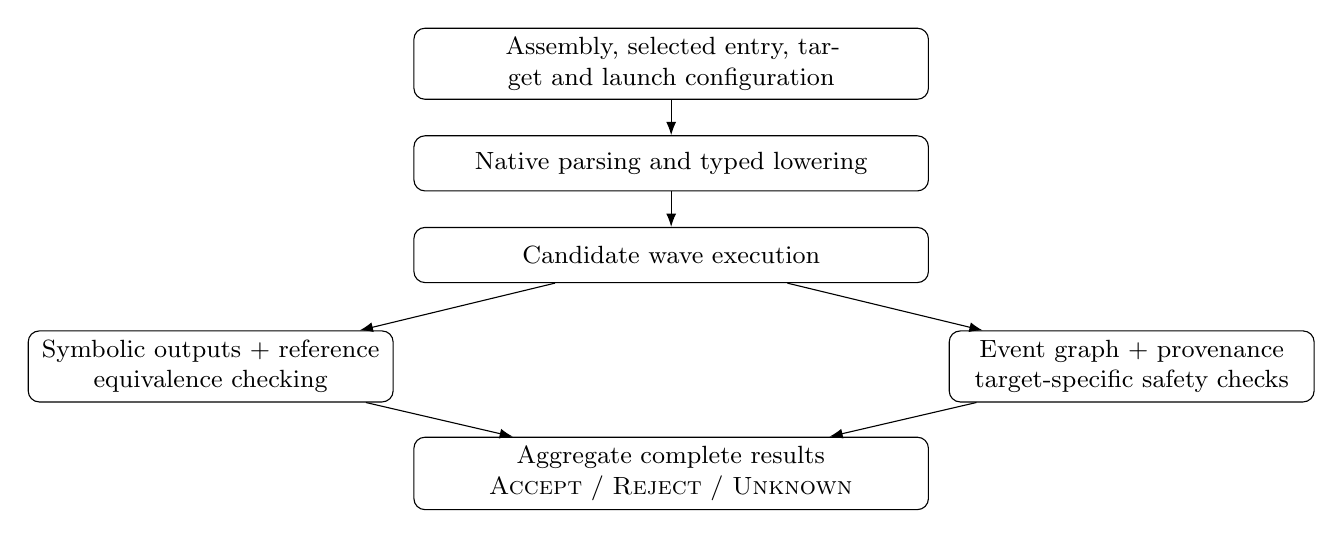
\begin{tikzpicture}[box/.style={draw,rounded corners,align=center,minimum height=0.7cm,
  text width=6.3cm,font=\small},smallbox/.style={box,text width=4.4cm},
  >={Latex},node distance=0.45cm]
\node[box] (source) {Assembly, selected entry, target and launch configuration};
\node[box,below=of source] (parse) {Native parsing and typed lowering};
\node[box,below=of parse] (exec) {Candidate wave execution};
\node[smallbox,below left=0.6cm and 0.25cm of exec] (expr) {Symbolic outputs + reference\\equivalence checking};
\node[smallbox,below right=0.6cm and 0.25cm of exec] (graph) {Event graph + provenance\\target-specific safety checks};
\node[box,below=1.95cm of exec] (result) {Aggregate complete results\\\accept{} / \reject{} / \unknown{}};
\draw[->] (source)--(parse);\draw[->] (parse)--(exec);
\draw[->] (exec)--(expr);\draw[->] (exec)--(graph);
\draw[->] (expr)--(result);\draw[->] (graph)--(result);
\end{tikzpicture}
\caption{Safety and mathematical equivalence consume separate artifacts. Kernel
comparison constructs and checks both kernels' execution graphs.}
\label{fig:pipeline}
\end{figure}

This boundary matters because candidate execution calculates asynchronous data
eagerly. The convenient value computed for a load does not establish that a
later instruction may safely consume it. Likewise, execution order in the
interpreter does not establish an ordering between conflicting hardware memory
effects. Graph checks must reconstruct the relevant justification from typed
issues, waits, source lifetimes and synchronization events.

\subsection{Result aggregation}

The aggregation rule is intentionally stronger than an arithmetic equality test.
For the compared outputs, acceptance requires a complete equivalence result and
a completed execution with every applicable graph property passing for every
kernel. A numeric refutation, output-index mismatch, failed property or deadlock
causes rejection. An unsupported instruction, resource limit, missing ordering
justification or unproved identity remains inconclusive unless another result
already refutes the run.

Let $I_a$ be the expected indices of checked array $a$ and $W_a$ its written
indices. Complete comparison requires $I_a=W_a$, in addition to equality of the
values at those indices. Equal counts are insufficient. Sampling can limit the
value expressions compared, but must not hide an absent or extra index or
replace the full element total with the sampled total. The CLI reports a combined
verdict. Python exposes separate graph, equivalence and element-count fields;
callers must inspect all of them for a complete result.

\section{Native parsing, lowering and launch reconstruction}
\label{sec:frontend}

\subsection{Assembly is a module, not a list of mnemonics}

The native frontend preserves target directives, code-object and metadata
versions, kernel descriptors, argument offsets and sizes, global objects,
labels, modifiers and source spans. Entry discovery must distinguish kernels
from unrelated helper functions without skipping unsupported instructions in an
actual entry. Unambiguous function bounds allow excluding a helper body;
overlapping definitions, ambiguous entry boundaries and fallthrough are errors.
Calls and arbitrary computed jumps remain outside the selected execution
profile.

Parsing checks the selected source forms, and lowering produces explicit typed
operations. Lowering validates caller-constructed modules as well as parsed
ones, so a direct Rust caller cannot bypass an instruction profile by changing
an architecture field. Legal register tuples, modifiers, address spaces,
immediates and source/destination widths are checked per form. An unknown
modifier cannot silently disappear. Instructions in unreachable or empty-EXEC
regions still need a legal supported encoding.

\subsection{AMDHSA changes the meaning of the launch}

The launch is reconstructed from both configuration and module metadata.
AMDHSA descriptors determine the initial register assignments and resource
budgets; argument metadata determines kernarg offsets and padding~\cite{llvmabi}.
Pointer and scalar arguments remain positional. Raw by-value arguments require
the exact bytes expected by the metadata, including caller-supplied padding.
Unsupported runtime-provided values must remain unavailable rather than
acquiring a convenient constant because workgroup zero is selected.

Packed local IDs, hidden grid inputs, static and dynamic LDS, module globals and
selected PC-relative relocations therefore require explicit models. Undefined
argument padding retains its definedness mask; a narrow valid consumer may use
the defined bits, while a consumer requiring missing bits stops. Unknown externs,
unsupported relocations and unavailable runtime state are reported rather than
invented. Target selection must agree with the source declaration.

\subsection{Physical state and predication}

A native wave has a shared PC and scalar state, with lane-indexed vector state.
EXEC selects active vector lanes; scalar instructions have their own behavior.
VCC and SCC are tracked explicitly, and undefined condition or carry state
cannot control a supported execution. gfx942/gfx950 retain 64 physical mask bits;
gfx1250 retains 32. Dependencies use physical register names and lane masks.
Value state preserves high/low-half definedness, while preserving an untouched
half creates an implicit whole-register read. The graph checks register-granule
hazards rather than modeling independent bit-level register lifetimes.

The implementation also distinguishes allocation from accessible encodings.
For example, a target may describe a larger logical VGPR allocation while the
selected instruction profile only handles encoded operands v0--v255. gfx1250
does not inherit an AGPR namespace from CDNA. These distinctions prevent a
well-formed-looking tuple from being interpreted through the wrong architecture.

\section{Values and byte-addressed storage}
\label{sec:values}

\subsection{Two arithmetic roles}

Address and concrete integer calculations need their native widths, signedness,
carry and wrapping behavior. Mathematical data feeds the shared expression DAG.
These roles cannot be exchanged freely: an abstract real is not an arbitrary
bit pattern, and an unconstrained data comparison cannot become a concrete
branch or pointer. Exact large integer constants must survive extraction and
serialization without passing through an imprecise floating representation.

Floating input/output storage has additional boundaries. F16, BF16 and FP8
encode data differently, and the implemented FP8 profiles vary by target.
Selected transport and concrete decoders preserve storage bits and conversion
points; symbolic mathematical operations preserve the stated real abstraction.
The implementation rejects incompatible numeric interpretations of the same
symbolic input identity. This avoids proving equality by treating a raw integer
word and a decoded floating value as the same variable.

Approximate hardware exponential idioms are represented by their supported
mathematical interpretation and disclosed assumptions. A mathematical identity
involving such an expression is not a bound on its hardware approximation
error. NaNs, exception behavior, subnormal modes and arbitrary IEEE rounding
remain outside the real-arithmetic proof.

\subsection{Memory width and definedness}

Global memory is byte-addressed, bounded and disjoint under the supplied launch.
Wide operations retain their complete memory footprint and constituent register
granules. A transfer that crosses an allocation boundary cannot be justified by
its starting address alone. Loads preserve which bits are defined; stores retain
their width and source dependencies. Partial-register updates must not initialize
an untouched half or erase a hazard on an overlapping half.

LDS has an aggregate target-specific bound. Assembly usually no longer describes
source-language subobjects, so an optional launch premise provides disjoint
named LDS ranges. When present, a complete DS or resolved-shared FLAT access must
fit one range as well as the aggregate allocation. The premise does not infer
padding, create initialized bytes or recover an unavailable source type. Its use
is recorded in provenance.

\subsection{Matrix instructions require explicit lane maps}

MFMA and WMMA consume distributed register fragments. A correct arithmetic
formula is insufficient unless each lane/item is mapped to the right matrix
coordinate and each output register receives the right result. For target maps
$a_t(\ell,r)=(i,k)$, $b_t(\ell,r)=(k,j)$ and $c_t(\ell,r)=(i,j)$, the interpreter
constructs
\[
 C'_{ij}=C_{ij}+\sum_k A_{ik}B_{kj}
\]
using the target's actual fragment coordinates. Source and accumulator roles,
register overlap, format, full-wave participation and supported modifiers are
part of the operation's contract.

CDNA MFMA and gfx1250 WMMA are separate implementations. The latter uses public
compiler/library lane layouts as an independent cross-check~\cite{flydsl}.
Basis-vector and asymmetric dense tests are useful because an all-zero matrix
cannot expose a transposed fragment or swapped lane. Tests also check accumulator
seeds, raw packed storage, complete output projections and harmful source/result
reuse. Native tensor-transfer descriptors have their own bounded 2D model and
issue-time capture; tensor copying does not itself establish publication.

\section{AMD safety is a target-specific protocol}
\label{sec:safety}

\subsection{Typed evidence and independent reconstruction}

The graph records instruction operands, memory issues and effects, completion
counter charges, register leases, matrix events and barrier state, together with
source provenance. Checkers first validate that a trace contains the evidence
required by its target and instruction profile. Missing or contradictory records
are inconclusive; absence of a witness is not automatically a passing trace.
An AMD event must not obtain a PTX certificate or a different AMD architecture's
rule through generic dispatch.

The native suite has four responsibilities: trace completeness; register/data
readiness; barrier generations and progress; and memory conflicts. Their typed
findings retain the issuing and consuming events for diagnostics and the viewer.
These checks are independent of mathematical output equality.
They validate typed record consistency rather than interpreting the assembly a
second time. The frontend and event producer remain responsible for the recorded
instruction values and memory addresses.

\subsection{Issue, completion and publication are different facts}

A memory instruction can issue before its data or source lifetime is ready for
reuse. gfx942/gfx950 charge VM/LGKM classes and check relevant matrix state
delays. Their wait thresholds certify a prefix only when the target's ordering
rules justify it; a mixed unordered class cannot acquire FIFO semantics from
its counter name alone. FLAT operations can impose more than one completion
obligation. LLVM's hazard recognizer provides a separately pinned reference for
selected matrix producer/consumer delays~\cite{llvmhazard}.

gfx1250 has separate Load, Store, DS, KM, X, asynchronous and Tensor accounting.
The X replay-source lifetime is tracked separately from data completion. An X
drain does not complete data; a data-completion wait also retires that operation's
translation lease, without draining unrelated operations. Tensor thresholds above zero remain
inconclusive in the selected profile. Public asynchronous and DMA descriptions
motivate this separation~\cite{llvmasync,llvmdma}; the precise implemented forms
are documented beside their fixtures.

After completion, a cross-wave consumer still needs valid publication and
execution order. A barrier does not create a missing memory completion. Cache
scope annotations do not create a barrier. The CDNA model's selected GLOBAL
publication rule additionally needs workgroup scope at both endpoints and its
single-CU workgroup premise. gfx1250's graph-level ordinary GLOBAL/resolved-global
FLAT write-dependency rule requires explicit system scope at both endpoints,
completion and a checked ordering relation. The current source profile exposes
that annotation for resolved-global FLAT; ordinary GLOBAL scope modifiers remain
unsupported. Neither rule establishes cross-workgroup race freedom.

Consider two waves sharing an LDS tile:
\begin{lstlisting}
producer: issue tile write -> wait for its completion -> arrive at barrier
consumer: arrive at barrier -> resume after valid release -> issue tile read
\end{lstlisting}
Removing the producer wait must not be repaired by the barrier. Removing the
barrier must not be repaired by the candidate interpreter happening to execute
the producer first. Reusing the producer's source register too early can violate
a separate lifetime obligation even if the eventual tile bytes look correct.

\subsection{Barrier identities, generations and lifetimes}

CDNA workgroup barriers are checked by wave participation and generation.
gfx1250 has separate unnamed split operations and selected allocated named
shader barriers. Named objects require physical ID, initialization incarnation,
phase, expected arrival count and explicit join/leave state. Reinitialization
must not revive an earlier lifetime or consume an old release. Program order
inside one wave cannot justify a noncommuting update from another wave.

For the unnamed object, END implicitly drops participation. An arrival that
contributes to a wait needs a completing wait execution-before the signaller's
END; candidate trace order alone cannot justify that relation. An arrival in a
phase with no participating wait does not create the same drop obligation.

The selected named SIGNAL model includes a nonzero M0 count update before the
arrival; zero preserves the existing count. NULL behavior is operation-specific,
and END does not implicitly drop named objects. The public synchronization model
distinguishes execution synchronization from memory visibility~\cite{llvmsync}.
Where pinned public descriptions disagree at the equal-to-existing-arrivals
boundary, the implementation remains inconclusive. Clustered and advanced
barrier modes outside the profile are rejected or unresolved, rather than
generalized from a nearby supported case.

\section{Reusing equivalence without weakening its inputs}
\label{sec:equivalence}

Native execution emits the same \code{SymbolicOutputs} representation consumed
by the existing specification and equivalence layers. The canonicalizer shares
and memoizes algebraic structure across kernels and output elements. Exact
coefficients, controlled session recycling and compact additive DAGs support
large native workloads without changing the intended identity being compared.
Term/resource limits still produce a failure to establish equivalence.

The input contract is as important as algebraic simplification. Array identities
and written indices must be unambiguous; duplicate output definitions cannot be
resolved by silently selecting the first. Dimension products and index arithmetic
must be checked before unfolding, because a wrapped size can otherwise turn a
large obligation into a vacuous empty one. Sampling must preserve the complete
footprint check and distinguish compared elements from all required elements.
These are shared safeguards for PTX and AMD.

Kernel-to-kernel comparison runs both safety branches. Expression exchange
files and VC dumps can replay mathematical comparisons without rerunning the
interpreter, but carry no execution-safety certificate. A replay equality must
therefore remain an equivalence-only result. Serialized outputs also need the
same identity and shape invariants as in-memory outputs.

The native workload ports retain logical dimensions, storage widths, strides,
masking, scalar arguments, scales and complete output coordinates. Different
wave geometry or a padded native tile can require an explicit projection of a
native superset. A smaller shape, fewer output arrays or a decoded-F32 substitute
is a different problem. NVIDIA-only descriptor/TMEM encodings are distinct from
portable obligations such as arithmetic, byte layout, lifetime and publication.

\section{Validation and reproducibility}
\label{sec:validation}

\subsection{Several kinds of evidence}

Validation uses a hierarchy of checks, each with a limited interpretation.
Compiler/assembler probes establish that an exact form can be emitted or
encoded. Frontend and lowering checks establish that the implementation accepts
that form. Symbolic execution and full graph checks establish properties of the
modeled trace. Full-output equivalence compares its mathematics. Independent
layout/numerical oracles and exact-assembly device runners test aspects that the
real-arithmetic model does not capture. No one level substitutes for another.

Positive controls use genuine compiler fixtures and complete configured
outputs. Negative controls remove a required wait or synchronization operation,
shift a footprint, corrupt a descriptor, or reuse a retained source. A negative
passes only when it reaches the intended typed failure; an unrelated parse error
or unsupported instruction is a separate outcome. Numerical experiments use
finite inputs and declared tolerances, and unsafe synchronization mutants are
kept in CPU analysis.

\begin{table}[ht]
\centering\small
\begin{tabular}{p{0.30\linewidth}p{0.19\linewidth}p{0.40\linewidth}}
\toprule
Artifact & Size & Interpretation \\
\midrule
Original workload registry & 32 registrations & Preserves original launch,
storage, specification and native projection contracts \\
Original output projection & 395,394 elements & Required coordinate set;
registry consistency is not an execution result \\
Full-workload compiler index & 7 modules; 185 mnemonics; 497 typed profiles &
Static forms, including each VOPD component; no ISA coverage percentage \\
Finite upstream feature mapping & 520 references & Pinned source/assertion/golden
relationships to actual native or shared tests and precise boundaries \\
\bottomrule
\end{tabular}
\caption{Finite artifact inventories in the accompanying implementation. Reference
files, kernel variants and instruction profiles are different counting units.}
\label{tab:artifacts}
\end{table}

These inventories are reproducible from manifests rather than inferred from
test-suite pass counts. Current reference files, assertion sources, goldens and
recursive test dependencies are bound by the generated mapping index. Default
validation detects drift; explicit regeneration after an intentional change
produces a reviewable source diff. That guards fixture identity, without
asserting that matching hashes prove execution correctness.

\subsection{Reproduction commands}

From the repository root, the common CPU checks are:
\begin{lstlisting}
cargo test --release --workspace
just test-python
python3 -m unittest discover -s tests/gfx1250/full-parity -p 'test_*.py'
python3 tests/gfx1250/full-parity/contract.py --require-all
python3 tests/gfx1250/full-parity/feature_contract.py
python3 tests/gfx1250/full-parity/validate_feature_mappings.py
python3 scripts/gfx950_parity.py summary --require-complete
\end{lstlisting}
The usage guide supplies a small runnable native copy example. Full-workload
CLI/Python runs, compiler regeneration and numerical device runs have separate
drivers and resource requirements. The default original-workload interface
tests select W01--W18; selecting every registered workload requires
\code{VOLTA_GFX1250_ORIGINAL_FULL=1}. Inventory counts in
Table~\ref{tab:artifacts} must not be read as a claim that a default test command
re-proves every full-size workload.

A small end-to-end check requires no device and compares all 65 copy outputs:
\begin{lstlisting}
cargo build --release -p volta_cli
target/release/volta verify \
  tests/gfx1250/fixtures/native-copy-add.s tests/gfx1250/specs/copy.spec \
  --backend amdgpu --target gfx1250 --kernel copy --block 65 --dim N=65 \
  --array x:0x10000:4:65:in --array out:0x30000:4:65:out \
  --param ptr:x --param ptr:out --param int:65
\end{lstlisting}

\subsection{Reading a successful run}

A useful result includes the exact source and launch, selected target,
execution terminal state, each graph property, complete output-index contract,
checked/total element counts, assumptions and final interface outcome. Logs and
device observations belong outside tracked fixture inputs. The browser viewer
shows wave width, source instructions, counter and barrier state, and typed
witness endpoints. Its bounded display selection never reduces the graph
analyzed by the checker, and its layout is not a hardware timing model.

\section{Limits and remaining work}
\label{sec:limits}

The main limitation is the semantic envelope. The analyzer examines one
configured workgroup and a candidate execution with concrete control, addresses
and synchronization parameters. It does not prove whole-grid behavior, arbitrary
input-dependent control, all scheduling behaviors, device faults or every ISA
encoding. Unsupported address spaces, calls, register encodings, tensor modes
and atomic profiles remain explicit boundaries.

The mathematical model omits general IEEE rounding and exceptional behavior.
Independent numerical testing can reveal a disagreement in tested inputs but
cannot turn a real-arithmetic identity into a universal floating-point theorem.
Similarly, compiler/assembler acceptance does not resolve an incomplete public
semantic description. Target-specific ambiguity must remain visible as
unsupported or unknown.

Implementation tests and code review are evidence, not a proof of the Rust
interpreter, event producer, checker or algebra engine. A useful next research
step is a formal account connecting native execution effects, completion and
publication to the graph contract. Further engineering work includes broader
instruction and runtime-state coverage, larger independent semantic corpora,
systematic differential testing and resource-efficient full-workload analysis.

\section{Conclusion}

Making Volta useful on AMD required retaining its expression-level comparison
while replacing the architecture-dependent path from assembly to justified
execution. The substantial work lies in ABI-defined state, physical wave and
register semantics, precise memory footprints, target-specific completion and
source lifetimes, barrier protocols and matrix lane maps. Independent graph
checking and exact output contracts connect those changes to a meaningful user
result. The resulting implementation supports a documented native subset with
reproducible controls and explicit limits; it does not transfer an NVIDIA
correctness theorem to AMD by changing an instruction decoder.

\appendix
\section{Source map}

\small
\begin{longtable}{p{0.29\linewidth}p{0.62\linewidth}}
\toprule
Concern & Source entry point \\
\midrule\endhead
Native syntax and AMDHSA metadata &
\repo{crates/volta_amdgpu_analysis/src/frontend/parse.rs}{frontend/parse.rs},
\repo{crates/volta_amdgpu_analysis/src/frontend/metadata.rs}{frontend/metadata.rs} \\
Typed instructions and target gates &
\repo{crates/volta_amdgpu_analysis/src/lower/mod.rs}{lower/mod.rs},
\repo{crates/volta_amdgpu_analysis/src/target.rs}{target.rs} \\
Wave execution and memory &
\repo{crates/volta_amdgpu_analysis/src/eval/interp.rs}{eval/interp.rs},
\repo{crates/volta_amdgpu_analysis/src/eval/memory.rs}{eval/memory.rs} \\
Encoded floating values and matrices &
\repo{crates/volta_amdgpu_analysis/src/eval/float_bits.rs}{eval/float\_bits.rs},
\repo{crates/volta_amdgpu_analysis/src/eval/matrix.rs}{eval/matrix.rs} \\
Typed native graph events &
\repo{crates/volta_graph/src/amdgpu.rs}{volta\_graph/src/amdgpu.rs} \\
CDNA and gfx1250 graph checks &
\repo{crates/volta_graph_check/src/amdgpu.rs}{graph\_check/src/amdgpu.rs},
\repo{crates/volta_graph_check/src/amdgpu/gfx1250.rs}{amdgpu/gfx1250.rs},
\repo{crates/volta_graph_check/src/amdgpu/gfx1250/named.rs}{gfx1250/named.rs} \\
Backend dispatch and verdict rules &
\repo{crates/volta_pipeline/src/backend.rs}{pipeline/src/backend.rs},
\repo{crates/volta_pipeline/src/aggregate.rs}{pipeline/src/aggregate.rs} \\
Output comparison and exchange &
\repo{crates/volta_equivalence/src/check.rs}{equivalence/src/check.rs},
\repo{crates/volta_equivalence/src/vc_dump.rs}{equivalence/src/vc\_dump.rs} \\
Specification and full footprint &
\repo{crates/volta_spec/src/instantiate.rs}{spec/src/instantiate.rs},
\repo{crates/volta_spec/src/spec.rs}{spec/src/spec.rs},
\repo{crates/volta_spec/src/footprint.rs}{spec/src/footprint.rs} \\
CLI, Python and viewer &
\repo{crates/volta_cli/src/main.rs}{CLI main.rs},
\repo{crates/volta_py/src/verify.rs}{Python verify.rs},
\repo{crates/volta_viz/src/export.rs}{viewer export.rs} \\
Full workload/output contracts &
\repo{tests/gfx1250/full/cases.json}{full/cases.json},
\repo{tests/gfx1250/full-parity/contract.py}{full-parity/contract.py} \\
Pinned public semantics &
\repo{tests/gfx1250/fixtures/semantic-references.json}{semantic-references.json},
\repo{docs/gfx942-graph-contract.md}{gfx942/gfx950 graph contract} \\
\bottomrule
\end{longtable}
\normalsize

\clearpage
\small\raggedright
\begin{thebibliography}{9}
\bibitem{volta}
Benjamin Driscoll, Kshitij Dubey, Anjiang Wei, Neeraj Kayal, Rahul Sharma and
Alex Aiken. \emph{Equivalence Checking of ML GPU Kernels}. OOPSLA 2026.
\href{https://arxiv.org/abs/2511.12638v3}{arXiv:2511.12638v3}.

\bibitem{cdna3}
AMD. \emph{AMD Instinct MI300 Instruction Set Architecture}.
\url{https://www.amd.com/content/dam/amd/en/documents/instinct-tech-docs/instruction-set-architectures/amd-instinct-mi300-cdna3-instruction-set-architecture.pdf}.

\bibitem{cdna4}
AMD. \emph{AMD CDNA4 Instruction Set Architecture Reference Guide}.
\url{https://www.amd.com/content/dam/amd/en/documents/instinct-tech-docs/instruction-set-architectures/amd-instinct-cdna4-instruction-set-architecture.pdf}.

\bibitem{llvmabi}
LLVM/ROCm contributors. \emph{User Guide for AMDGPU Backend}.
Revision \code{5fd50ec8e07abb94e203933017e8d6e40fb51824}.
\href{https://github.com/ROCm/llvm-project/blob/5fd50ec8e07abb94e203933017e8d6e40fb51824/llvm/docs/AMDGPUUsage.md}{AMDGPUUsage.md}.

\bibitem{llvmhazard}
LLVM contributors. \emph{GCNHazardRecognizer.cpp}, LLVM 22.1.0,
revision \code{4434dabb69916856b824f68a64b029c67175e532}.
\href{https://github.com/llvm/llvm-project/blob/4434dabb69916856b824f68a64b029c67175e532/llvm/lib/Target/AMDGPU/GCNHazardRecognizer.cpp}{Pinned source}.

\bibitem{llvmsync}
LLVM/ROCm contributors. \emph{AMDGPU Execution Synchronization}.
Revision \code{5fd50ec8e07abb94e203933017e8d6e40fb51824}.
\href{https://github.com/ROCm/llvm-project/blob/5fd50ec8e07abb94e203933017e8d6e40fb51824/llvm/docs/AMDGPUExecutionSynchronization.md}{Pinned document}.

\bibitem{llvmasync}
LLVM/ROCm contributors. \emph{AMDGPU Asynchronous Operations}.
Revision \code{5fd50ec8e07abb94e203933017e8d6e40fb51824}.
\href{https://github.com/ROCm/llvm-project/blob/5fd50ec8e07abb94e203933017e8d6e40fb51824/llvm/docs/AMDGPUAsyncOperations.md}{Pinned document}.

\bibitem{llvmdma}
LLVM/ROCm contributors. \emph{AMDGPU DMA Operations}.
Revision \code{5fd50ec8e07abb94e203933017e8d6e40fb51824}.
\href{https://github.com/ROCm/llvm-project/blob/5fd50ec8e07abb94e203933017e8d6e40fb51824/llvm/docs/AMDGPUDMAOperations.md}{Pinned document}.

\bibitem{flydsl}
ROCm FlyDSL contributors. \emph{GFX1250 WMMA Layout and Matrix Atoms}.
Revision \code{f37f7a2b98f295902240f9f96612222003578b40}.
\href{https://github.com/ROCm/FlyDSL/blob/f37f7a2b98f295902240f9f96612222003578b40/lib/Dialect/FlyROCDL/GFX1250/WmmaLayout.h}{WmmaLayout.h} and
\href{https://github.com/ROCm/FlyDSL/blob/f37f7a2b98f295902240f9f96612222003578b40/lib/Dialect/FlyROCDL/GFX1250/MmaAtom.cpp}{MmaAtom.cpp}.
\end{thebibliography}
\end{document}
